\part{More on complexity}
\frame{\partpage}

\begin{frame}{Common complexity classes}
	\begin{center}
		\begin{tabular}{clc}
			\pause ``Faster'' & Constant & $O(1)$ \\
			\pause $\uparrow$ & Logarithmic & $O(\log n)$ \\
			\pause $|$ & Fractional power & $O(n^k)$, $k < 1$ \\
			\pause $|$ & Linear & $O(n)$ \\
			\pause $|$ & Quadratic & $O(n^2)$ \\
			\pause $|$ & Polynomial & $O(n^k)$, $k > 1$  \\
			\pause $\downarrow$ & Exponential & $O(e^n)$ \\
			\pause ``Slower'' & Factorial & $O(n!)$
		\end{tabular}
	\end{center}
\end{frame}

\begin{frame}{Common complexity classes}
	\begin{center}
		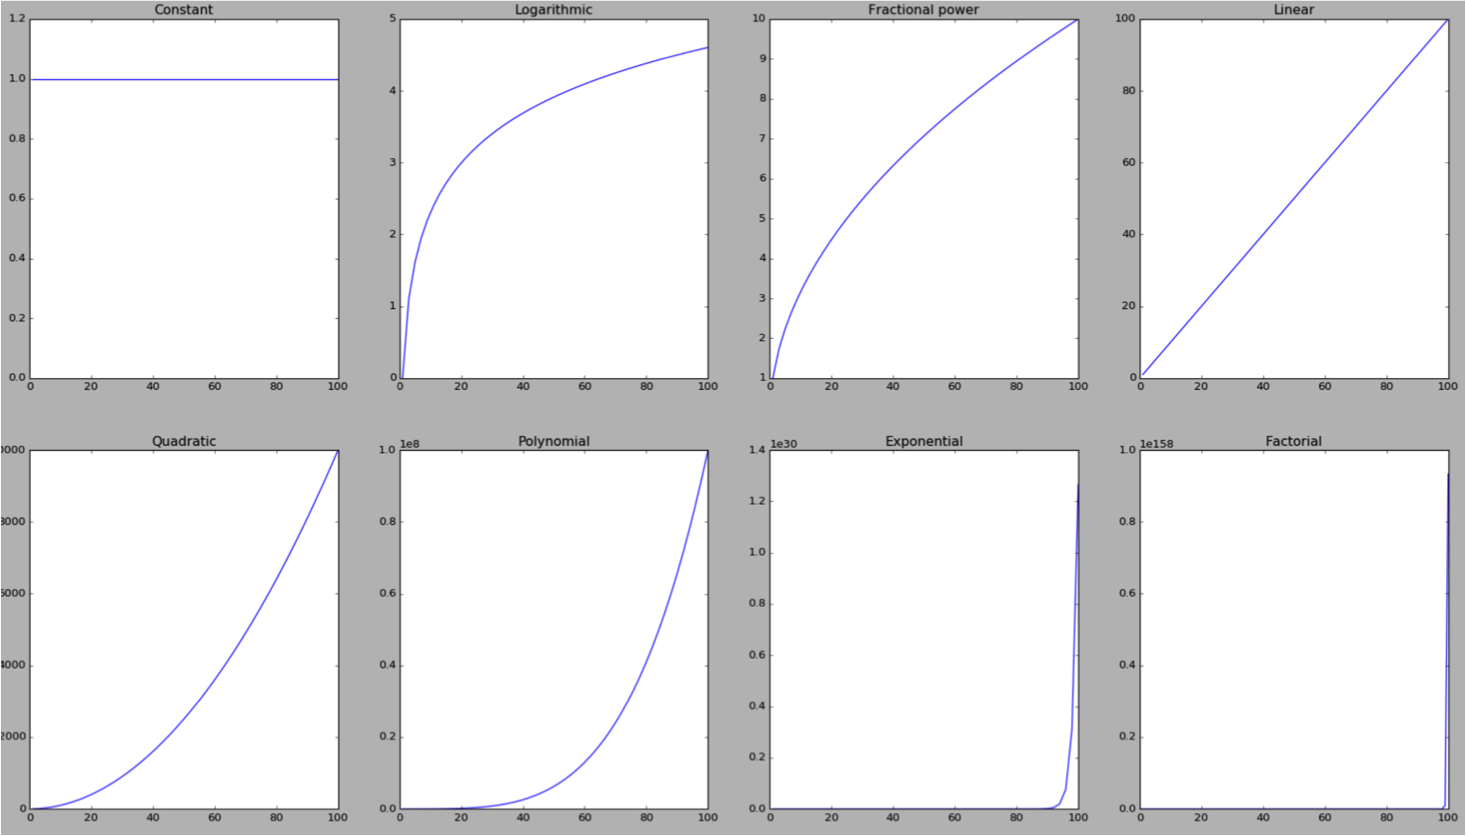
\includegraphics[width=\textwidth]{complexity_classes}
	\end{center}
\end{frame}

\begin{frame}{Working with big $O$ notation}
	\begin{itemize}
		\pause\item Can ignore \textbf{leading constants}
			\begin{itemize}
				\pause\item If one algorithm takes $n^2$ operations,
					another takes $500n^2$
					and a third takes $0.00000001n^2$,
					all three are $O(n^2)$
			\end{itemize}
		\pause\item Take only the \textbf{dominant term}
			\begin{itemize}
				\pause\item The term that is largest when $n$ is large
				\pause\item If an algorithm takes $0.1n^3 + 300n^2 + 7000$ operations,
					it is $O(n^3)$
			\end{itemize}
		\pause\item Multiply \textbf{compound} algorithms
			\begin{itemize}
				\pause\item If an algorithm does $n$ ``things'' and each ``thing'' is $O(n)$,
					then the overall algorithm is $O(n^2)$
			\end{itemize}
	\end{itemize}
\end{frame}

\begin{frame}{Quadratic complexity}
	\begin{columns}
		\begin{column}{0.4\textwidth}
			\only<3->{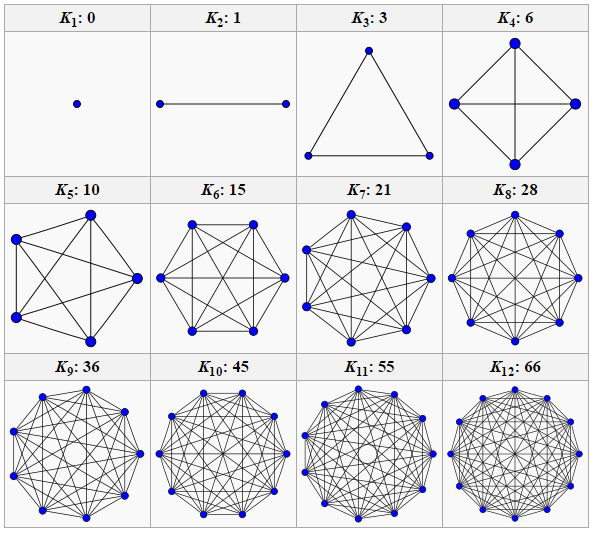
\includegraphics[width=\textwidth]{complete_graph}}
		\end{column}
		\begin{column}{0.6\textwidth}
			\begin{itemize}
				\item Collision detection between $n$ objects \pause
				\item The na\"ive way: check \textbf{each pair} of objects to see whether they have collided \pause
				\item This is \textbf{quadratic} or $O(n^2)$ \pause
				\item Doubling the number of objects would \textbf{quadruple} the time required! \pause
				\item Cleverer methods exist that are more scalable \pause
					\begin{itemize}
						\item Further reading: spatial hashing, quadtrees, octrees, Verlet lists
					\end{itemize}
			\end{itemize}
		\end{column}
	\end{columns}
\end{frame}

\begin{frame}{Exponential complexity}
	\begin{itemize}
		\pause\item A \text{prime number} is a number that is divisible only by $1$ and itself
		\pause\item Given an $n$-bit number $m = pq$ that is a product of two primes $p$ and $q$, find $p$ and $q$.
	\end{itemize}
	\pause
	\begin{algorithmic}
		\For{$p = 2, 3, \dots, m$}
			\State $q \gets m / p$
			\If{$q$ is an integer}
				\State \textbf{return} $p,q$
			\EndIf
		\EndFor
	\end{algorithmic}
	\begin{itemize}
		\pause\item Since $m \leq 2^n-1$, in the worst case this is $O(2^n)$
			\begin{itemize}
				\pause\item Actually even slower because division is not $O(1)$
			\end{itemize}
		\pause\item Adding 1 to $n$ potentially \textbf{doubles} the running time!
	\end{itemize}
\end{frame}

\begin{frame}{Aside: a famous unanswered question in computing}
	\begin{itemize}
		\pause\item A problem is ``in $P$'' if it can be solved with an
			algorithm running in $O(n^k)$ time
		\pause\item A problem is in $NP$ if a potential solution can be checked in $O(n^k)$ time
			\begin{itemize}
				\pause\item Equivalently, it can be solved with an algorithm running in $O(n^k)$ time on an infinitely parallel machine
			\end{itemize}
		\pause\item Are there any problems in $NP$ but not in $P$?
	\end{itemize}
\end{frame}

\begin{frame}{P versus NP}
	\begin{itemize}
		\pause\item If you can find a \textbf{mathematical proof} that either $P = NP$ or $P \neq NP$, there's a \$1 million prize...
		\pause\item It is believed that $P \neq NP$, so large instances of
			$NP$-hard problems are not solvable in a feasible amount of time
			\begin{itemize}
				\pause\item Many types of cryptography are based on this assumption
				\pause\item Quantum computers are ``infinitely parallel'' in a sense
					so \emph{can} solve some large $NP$-hard problems
			\end{itemize}
	\end{itemize}
\end{frame}

\begin{frame}{Caveats}
	\begin{itemize}
		\item Time complexity only tells us how an algorithm \textbf{scales} with the size of the input \pause
			\begin{itemize}
				\item If we know the input will always be \textbf{small}, time complexity is not so important \pause
				\item Linear search is quicker than binary search if you only ever have 3 elements \pause
				\item Na\"ive collision detection is fine if your game only ever has 4 objects on screen \pause
				\item Sometimes complexity in terms of other resources (e.g.\ space, bandwidth) are more important than time \pause
			\end{itemize}
		\item Software development is all about choosing \textbf{the right tool for the job} \pause
			\begin{itemize}
				\item If you need scalability, choose a scalable algorithm \pause
				\item Otherwise, choose simplicity
			\end{itemize}
	\end{itemize}
\end{frame}

\begin{frame}{Summary}
	\begin{itemize}
		\item Time complexity tells us how the running time of an algorithm \textbf{scales} with the size of the data
			it is given \pause
		\item Choice of data structures and algorithms can have a large impact on the efficiency of your software \pause
		\item ... but only if scalability is actually a factor
	\end{itemize}
\end{frame}
